\chapter{Micro-management}
\begin{quotation}
\noindent
\textit{La vie est la somme de tous vos choix.
\vspace{0.2cm}\\
Life is the sum of all your choices.}
%\vspace{0.2cm}\\
\begin{flushright}Albert Camus\end{flushright}
\end{quotation}

\lettrine{W}{e} present a Bayesian sensory-motor model for multi-agent (decentralized) units control in an adversarial setting. Orders, coming from higher up in the decision hierarchy, are integrated as another sensory input. We evaluated our model on classic StarCraft \glos{micro} tasks. This work was published in \citep{SYNNAEVE:Micro}.

\chaptertoc
\newacronym{RL}{RL}{reinforcement learning}

\begin{itemize}
\item \underline{Problem:} optimal control of units in a (real-time) huge adversarial actions space (collisions, accelerations, terrain, damages, areas of effects, foes, goals...).
\item \underline{Problem that we solve:} efficient coordinated control of units incorporating all low level actions and inputs, plus higher level orders and representations.
\item \underline{Type:} it is a problem of \textit{multi-agent control in an adversarial environment}\footnote{Strictly, it can be modeled as a \glos{pomdp} for each unit independently with $S$ the states of all the other units (enemies and allied altogether) which are known through observations $O$ by conditional observations probabilities $\Omega$, with $A$ the set of actions for the given unit, $T$ transition probabilities between states and depending on actions, and the reward function $R$ based on goal execution, unit survivability and so on... It can also be viewed as a (gigantic) \glos{pomdp} solving the problem for all (controlled units) at once, the advantage is that all states $S$ for allied units is known, the disadvantage is that the combinatorics of $T$ and $A$ make it intractable for useful problems.}.
\item \underline{Complexity:} \textsc{pspace}-complete \citep{Papadimitriou87,GamingComplexity}. Our solutions are real-time on a laptop.
\end{itemize}

% TODO: 
% add graphical model??\\

\begin{figure}[ht]
\begin{center}
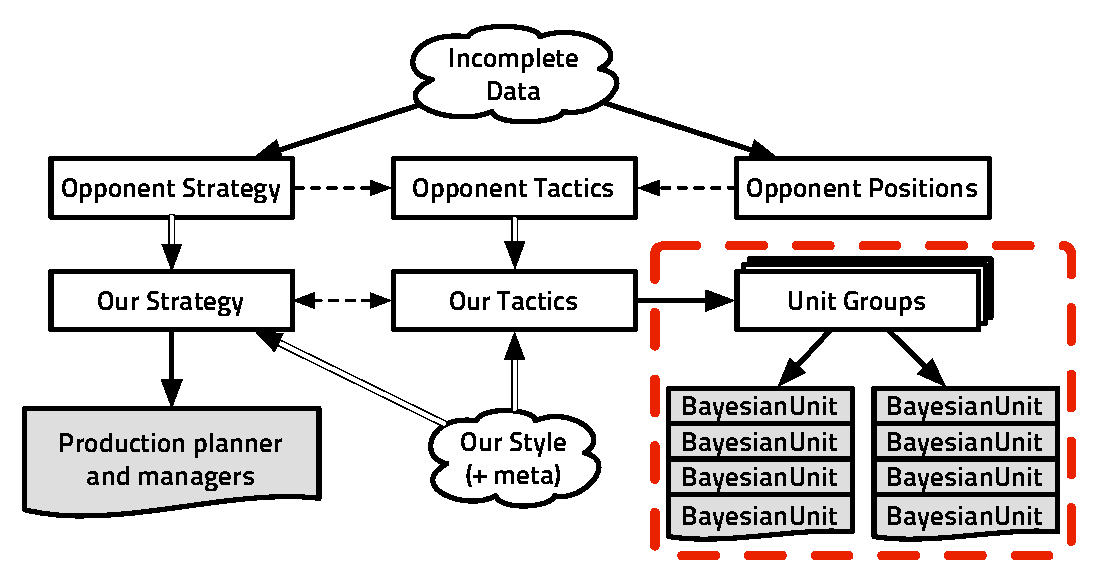
\includegraphics[width=13cm]{images/starcraft_bbq_concept_MICRO.pdf}
\end{center}
\caption{Information-centric view of the architecture of the bot, the part concerning this chapter (\glos{micro}) is in the dotted rectangle}
\label{fig:conceptMICRO}
\end{figure}

\section{Units Management}
In this part, we focus on \glos{micro}, which is the lower-level in our hierarchy of decision-making levels (see Fig.~\ref{fig:starcraft_abstraction_time}) and directly affect units control/inputs. Micro-management consists in maximizing the effectiveness of the units \textit{i.e.} the damages given/damages received ratio. These has to be performed simultaneously for units of different types, in complex battles, and possibly on heterogeneous terrain. 
For instance: retreat and save a wounded unit so that the enemy units would have to chase it either boosts your firepower (if you save the unit) or weakens the opponent's (if they chase). 
Let $\mathbf{U}$ be the set of the $m$ units to control, $\mathbf{A} = \{\cup_i\ \vec{d_i}\} \cup \mathbf{S}$ be the set of possible actions (all $n$ possible $\vec{d}$ directions, standing ground included, and $\mathbf{S}$kills, firing included), and $\mathbf{E}$ the set of enemies. As $|\mathbf{U}| = m$, we have $|\mathbf{A}|^{m}$ possible combinations each turn, and the enemy has $|\mathbf{A}|^{|\mathbf{E}|}$. 
The dimension of the set of possible actions each micro-turn (for instance: 1/24th of a second in StarCraft) constrains reasoning about the state of the game to be hierarchical, with different levels of granularity. In most RTS games, a unit can go (at least) in its 24 surrounding tiles (see Figure~\ref{fig:sc_fight}, each arrow correspond to a $\vec{d_i}$)
) %, combination of N, S, E, W up to the 2nd order), 
stay where it is, attack, and sometimes cast different spells: which yields more than 26 possible actions each turn. Even if we consider only 8 possible directions, stay, and attack, with $N$ units, there are $10^N$ possible combinations each turn (all units make a move each turn). As large battles in StarCraft account for \textit{at least} 20 units on each side, optimal units control hides in too big a search space to be fully explored in real-time (sub-second reaction at least) on normal hardware, even if we take only one decision per unit per second.

\begin{figure}
\begin{center}
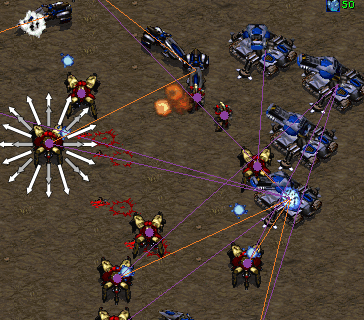
\includegraphics[width=8.6cm]{images/SC_fight_3b.png}
\end{center}
\caption{Screen capture of a fight in which our bot controls the bottom-left units in StarCraft. The 25 possible directions ($\vec{d_1} \dots \vec{d_{25}}$) are represented for a unit with white and grey arrows around it. Orange lines represent units' targets, purple lines represent units' priority targets (which are objective directions in \textit{fightMove()} mode).}
\label{fig:sc_fight}
\end{figure}

Our distributed sensory-motor model for \glos{micro} is able to handle both the complexity of unit control and the need of hierarchy (see Figure~\ref{fig:conceptMICRO}, this chapter focuses on the part inside the dotted line). We treat the units independently, thus reducing the complexity (no communication between our ``Bayesian units''), and allows to take higher-level orders into account along with local situation handling. For instance: the tactical planner may decide to retreat, or go through a choke under enemy fire, each Bayesian unit will have the higher-level order as a sensory input, along with topography, foes and allies positions. From its perception, our Bayesian robot \citep{Lebeltel04} can compute the distribution over its motor control. The performances of our models are evaluated against the original StarCraft AI and a reference AI (based on our targeting heuristic): they have proved excellent in this benchmark setup.


\section{Related Works}
Technical solutions include finite states machines (FSM) \citep{FSM}, genetic algorithms (GA) \citep{GA,Bakkes04,teamCompositionRTS}, reinforcement learning (RL) \citep{Marthi05concurrenthierarchical,Madeira06}, case-based reasoning (CBR) \citep{LTW,CBR-RL}, continuous action models \citep{Molineaux08}, reactive planning \citep{WeberCIG10}, upper confidence bounds tree (UCT) \citep{UCT}, potential fields \citep{Hagelback2009}, influence maps\citep{teamCompositionRTS}, and cognitive human-inspired models \citep{SORTS}.

FSM are well-known and widely used for control tasks due to their efficiency and implementation simplicity. However, they don't allow for state sharing, which increases the number of transitions to manage, and state storing, which makes collaborative behavior hard to code \citep{Cutumisu09}. Hierarchical FSM (HFSM) solve some of this problems (state sharing) and evolved into behavior trees (BT, hybrids HFSM) \citep{Isla} and behavior multi-queues (resumable, better for animation) \citep{Cutumisu09} that conserved high performances. %%%All these architectures does not include mechanisms to receive orders from separate entities. For instance, our strategic leader and tactical planners should be part of the (hierarchical) state machine, down to the control of units, which is not very flexible. 
However, adaptivity of behavior by parameters learning is not the main focus of these models, and unit control is a task that would require a huge amount of hand tuning of the behaviors to be really efficient. 
Also, these architectures does not allow reasoning under uncertainty, which helps dealing with local enemy and even allied units. Our agents see local enemy (and allied) units but do not know what action they are going to do. They could have perfect information about the allied units intentions, but this would need extensive communication between all the units.

Some interesting uses of \glos{RL} \citep{Sutton} to RTS research are concurrent hierarchical (units Q-functions are combined higher up) \glos{RL} \citep{Marthi05concurrenthierarchical} to efficiently control units in a multi-effector system fashion. \cite{Madeira06} advocate the use of prior domain knowledge to allow faster \glos{RL} learning and applied their work on a large scale (while being not as large as StarCraft) turn-based strategy game. In real game setups, \glos{RL} models have to deal with the fact that the state spaces to explore is enormous, so learning will be slow or shallow. It also requires the structure of the game to be described in a partial program (or often a partial Markov decision process) and a shape function \citep{Marthi05concurrenthierarchical}. RL can be seen as a transversal technique to learn parameters of an underlying model, and this underlying behavioral model matters. \cite{GA} used evolutionary learning techniques, but face the same problem of dimensionality. 

Case-based reasoning (CBR) allows for learning against dynamic opponents \citep{LTW} and has been applied successfully to strategic and tactical planning down to execution through behavior reasoning rules \citep{Ontanon2007}. CBR limitations (as well as RL) include the necessary approximation of the world and the difficulty to work with multi-scale goals and plans. These problems led respectively to continuous action models \citep{Molineaux08}and reactive planning \citep{WeberCIG10}. Continuous action models combine RL and CBR. Reactive planning use a decomposition similar to hierarchical task networks \citep{HTNPlanning} in that sub-plans can be changed at different granularity levels. Reactive planning allows for multi-scale (hierarchical) goals/actions integration and has been reported working on StarCraft, the main drawback is that it does not address uncertainty and so can not simply deal with hidden information (both extensional and intentional). 
Fully integrated FSM, BT, RL and CBR models all need vertical integration of goals, which is not very flexible (except in reactive planning).

Monte-Carlo planning \citep{Chung05} and upper Upper 
confidence bounds tree (UCT) planning (coming from Go AI) \citep{UCT} 
 samples through the (rigorously intractable) plans space by 
incrementally building the actions tree through Monte-Carlo sampling. 
UCT for tactical assault planning \citep{UCT} in RTS does not require to encode human knowledge (by opposition to Monte-Carlo planning) but it is too costly, both in learning and running time, to go down to units control on RTS problems. 
Our model subsumes potential fields \citep{Hagelback2009}, which are powerful and used in new generation RTS AI to handle threat, as some of our Bayesian unit sensory inputs are potential damages and tactical goodness (height for the moment) of positions. \cite{HagelbackJ08} presented a multi-agent potential fields based bot able to deal with fog of war in the Tankbattle game. \cite{Avery09} and \cite{SmithCIG10} co-evolved influence map trees for spatial reasoning in RTS games. \cite{Danielsiek_2008} used influence maps to achieve intelligent squad movement to flank the opponent in a RTS game. A drawback for potential field-based techniques is the large number of parameters that has to be tuned in order to achieve the desired behavior. 
Our model provides flocking and local (subjective to the unit) influences on the pathfinding as in \citep{teamCompositionRTS}, which uses self-organizing-maps (SOM). In their paper, Preuss \textit{et al.} are driven by the same quest for a more natural and efficient behavior for units in RTS. 
We would like to note that potential fields and influence maps are reactive control techniques, and as such, they do not perform any form of lookahead. In their raw form (without specific adaptation to deal with it), they can lead units to be stuck in local optimums (potential wells). 


Pathfinding is used differently in planning-based approaches and reactive approaches. \cite{Danielsiek_2008} is an example of the permeable interface between pathfinding and reactive control with influence maps augmented tactical pathfinding and flocking. As we used pathfinding as the mean to get a sensory input towards the objective, we were free to use a \textit{low resolution} and \textit{static} pathfinding for which A* was enough. Our approach is closer to the one of \citep{Reynolds_1999}: combining a simple path for the group with flocking behavior. In large problems and/or when the goal is to deal with multiple units pathfinding taking collisions (and sometimes other tactical features), more efficient, incremental and adaptable approaches are required. 
Even if specialized algorithms, such as D*-Lite \cite{KoenigL02} exist, it is most common to use A* combined with a map simplification technique that generates a simpler navigation graph to be used for pathfinding. An example of such technique is Triangulation Reduction A*, that computes polygonal triangulations on a grid-based map \cite{Demyen_2006}. In recent commercial RTS games like Starcraft 2 or Supreme Commander 2, flocking-like behaviors are inspired of continuum crowds (``flow field'') \cite{Treuille2006}. A comprehensive review about (grid-based) pathfinding was recently done by Sturtevant \cite{sturtevant2012benchmarks}.


Finally, there are some cognitive approaches to RTS AI \citep{SORTS}, and we particularly agree with Wintermute \textit{et al.} analysis of RTS AI problems. Our model has some similarities: separate agents for different levels of abstraction/reasoning and a perception-action approach (see Figure~\ref{fig:conceptMICRO}).

\section{A Pragmatic Approach to Units Control}
\subsection{Action and Perception}
\subsubsection{Movement}
The possible actions for each unit are to move from where they are to wherever on the map, plus to attack and/or use special abilities or spells. Atomic moves (shown in Fig.~\ref{fig:sc_fight} by white and gray plain arrows) correspond to move orders which will make the unit go in a straight line and \textit{not} call the pathfinder (if the terrain is unoccupied/free). There are collisions with buildings, other units, and the terrain (cliffs, water, etc.) which denies totally some movements for ground units. Flying units do not have any collision (neither with units, nor with terrain obviously). When a \textit{move order} is issued, if the selected position is further than atomic moves, the pathfinder function will be called to decide which path to follow. We decided to use only atomic (i.e. small and direct) moves for this reactive model, using other kinds of moves is discussed later in perspectives.

\subsubsection{Attacks}
To attack another unit, a given unit has to be in range (different attacks or abilities have different ranges) it has to have reloaded its weapon, which can be as quick as 4 times per second up to $\approx$3 seconds (75 frames) per attack. To cast a spell or use an ability also requires energy, which (re)generates slowly and can be accumulated up to a limited amount. Also, there are different kinds of attacks (normal, concussive, explosive), which modify the total amount of damages made on different types of units (small, medium, big), and different spread form and range of splash damages. Some spells/abilities absorb some damages on a given unit, others make a zone immune to all range attacks, etc. Finally, ranged attackers at a lower level (in terrain elevation) than their targets have an almost 50\% miss rate. These reasons make it an already hard problem just to select what to do without even moving. 

\subsubsection{Perceptions: potential damage map}
Perceptions are of different natures: either they are direct measurements inside the game, or they are built up from other direct measurements or even come from our AI higher level decisions. Direct measurements include the position of terrain elements (cliffs, water, space, trees). Built up measurements comes from composition of informations like the potential damage map (see Fig.~\ref{fig:potential_damage_map}. We maintain two (ground and air) damage maps which are built by summing all enemy units attack damages, normalized by their attack speed, for all positions which are in their range. These values are then discretized in levels $\{No, Low, Medium, High\}$ relative to the hit (health) points (HP) of the unit that we are moving. For instance, a tank (with many HP) will not fear going under some fire so he may have a $Low$ potential damages value for a given direction which will read as $Medium$ or $High$ for a light/weak unit like a marine. This will act as subjective potential fields \citep{Hagelback2009} in which the (repulsive) influence of the potential damages map depends on the unit type. The discrete steps are: 
$$\left\{0, \llbracket 0\dots \frac{unit\ base\ HP}{2}\rrbracket, \rrbracket \frac{unit\ base\ HP}{2} \dots unit\ base\ HP\llbracket, \llbracket unit\ base\ HP \dots +\inf\llbracket\right\}$$

\begin{figure}[h]
\begin{center}
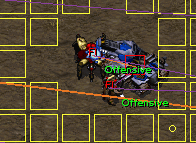
\includegraphics[width=4cm]{images/tank_cac.png}
\hspace{1cm}
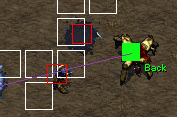
\includegraphics[width=4cm]{images/kiting.png}
\caption{Potential damage map (white squares for low potential damages, and yellow square for moderate potential damages). Left: we can see that the tank in siege mode (big blue unit with a red square on top) cannot shoot at close range and thus our units (in red) were attracted to the close safe zone. Right: the enemy units (blue, with red squares on top) are contact attack units and thus our unit (red, with a plain green square on top) is ``kiting'' (staying out of range): attacking and then retreating away (out of their range).}
\end{center}
\label{fig:potential_damage_map}
\end{figure}

\subsubsection{Repulsion/attraction}
For repulsion/attraction between units (allied or enemies), we could consider the instantaneous position of the units but it would lead to squeezing/expanding effects when moving large groups. Instead, we use their interpolated position at the time at which the unit that we move will be arrived in the direction we consider. In the right diagram in Figure~\ref{ fig:BayesianUnit_perceptions}, we want to move the unit in the center (\texttt{U}). There is an enemy (\texttt{E}) unit twice as fast as ours and an allied unit (\texttt{A}) three times as ours. When we consider moving in the direction just above us, we are on the interpolated position of unit \texttt{E} (we travel one case when they do two); when we consider moving in the direction directly on our right (East), we are on the interpolated position of unit \texttt{A}. 
We consider where the unit will be $\frac{\mathrm{dist}(unit, \vec{d_i})}{unit.speed}$ time later, but also its size (some units produce collisions in a smaller scale than our discretization).

\subsubsection{Objective}
The goals coming from the tactician model (see Fig.~\ref{fig:conceptMICRO}) are broken down into steps which gives objectives to each units. The way to incorporate the objective in the reactive behavior of our units is to add an attractive sensory input. This objective is a fixed direction $\vec{o}$ and we consider the probabilities of moving our unit in $n$ possible directions $\vec{d_1} \dots \vec{d_n}$ (in our StarCraft implementation: $n=25$ atomic directions). To decide the attractiveness of a given direction $\vec{d_i}$ with regard to the objective $\vec{o}$, we consider a weight which is proportional to the dot product $<\vec{o},\vec{d_i}>$, with a threshold minimum probability, as shown in Figure~\ref{fig:BayesianUnit_perceptions}.

\begin{figure}[h]
\begin{center}
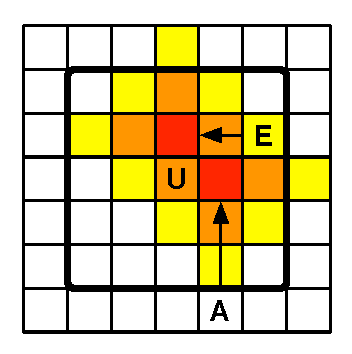
\includegraphics[width=4.5cm]{images/repulsion_units_interpolation.pdf}
\hspace{1cm}
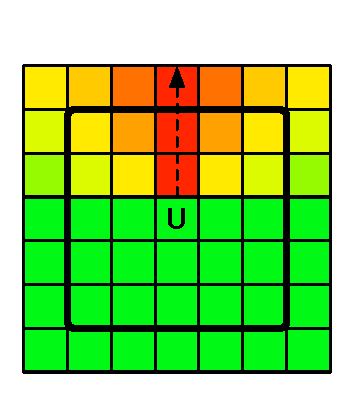
\includegraphics[width=4.5cm]{images/obj_Bayesian_units.pdf}
\caption{In both figures, the thick squares represents the boundaries of the 24 atomic directions (25 small squares with the current unit position) around the unit (\texttt{U}). Red is high probability, down to green low probability. Left: repulsion of the linear interpolation of the trajectories (here with uncertainty) of enemy unit (\texttt{E}) and allied unit (\texttt{A}), depending on their speed. Right: attraction of the objective (in direction of the dotted arrow) which is proportional to dot-product of the direction (square) considered, with a minimum threshold (in green).}
\label{fig:BayesianUnit_perceptions}
\end{center}
\end{figure}


\subsection{A Simple Unit}
\subsubsection{Greedy pragmatism}
Is staying alive better than killing an enemy unit? Is a large splash damage better than killing an enemy unit? Is it better to fire or move? In that event, where? Even if we could compute to the end of the fight and apply the same approach that we have for board games, how do we infer the best ``set of next moves'' for the enemy? %when the space of possible moves is so huge and the number of possible reasoning methods %(sacrifices and influences of other parts of the game for instance) 
%is bigger than for Chess? 
For enemy units, it would require exploring the tree of possible plans (intractable) whose we could at best only draw samples from \citep{UCT}. Even so, taking enemy minimax (to which depth?) moves for facts would assume that the enemy is also playing minimax (to the same depth) following exactly the same valuation rules as ours. Clearly, RTS \glos{micro} is more inclined to reactive planning than board games reasoning. That does not exclude having higher level (strategic and tactic) goals. In our model, they are fed to the unit as sensory inputs, that will have an influence on its behavior depending on the situation/state the unit is in. 
We should at least have a model for higher-level decisions of the enemy and account for uncertainty of moves that could be performed in this kind of minimax approach. So, as complete search through the min/max tree is intractable, we propose a first simple solution: have a greedy target selection heuristic leading the movements of units to benchmark our Bayesian model against. In this solution, each unit can be viewed as an effector, part of a multi-body (multi-effector) agent, grouped under a units group. 

\subsubsection{Targeting heuristic}
The idea behind the heuristic used for target selection is that units need to focus fire (which leads to less incoming damages if enemy units die faster) on units that do the most damages, have the less hit points, and take the most damages from their attack type. This can be achieved by using a data structure, shared by all our units engaged in the battle, that stores the damages corresponding to future allied attacks for each enemy units. Whenever a unit will fire on a enemy unit, it registers there the future damages on the enemy unit. As attacks are not all instantaneous and there are reload times, it helps focus firing greatly\footnote{The only degenerated case would be if all our units register their targets at once (and all the enemy units have the same priority) and it never happens (plus, units fire rates have a randomness factor).}. 
We also need a set of priority targets for each of our unit types that can be drawn from expert knowledge or learned (reinforcement learning) battling all unit types. A unit select its target among the most focus fired units with positive future hit point (current hit points minus registered damages), while prioritizing units from the priority set of its type. The units group can also impose its own priorities on enemy units (for instance to achieve a goal). The target selection heuristics is fully depicted in \ref{alg:targetselection} in the appendices.

\subsubsection{Fight behavior}
Based on this targeting heuristic, we design a very simple FSM based unit as shown in Figure~\ref{fig:fight_FSM} and Algorithm~\ref{alg:fight_FSM}: when the unit is not firing, it will either flee damages if it has taken too much damages and/or if the differential of damages is too strong, or move to be better positioned in the fight (which may include staying where it is). In this simple unit, the \textit{flee()} function just tries to move the unit in the direction of the biggest damages gradient (towards lower potential damages zones). The \textit{fightMove()} function tries to position the units better: in range of its priority target, so that if the priority target is out of reach, the behavior will look like: ``try to fire on target in range, if it cannot (reloading or no target in range), move towards priority target''. As everything is driven by the firing heuristic (that we will also use for our Bayesian unit), we call this AI the Heuristic Only AI (HOAI).

\begin{figure}[h]
\begin{algorithmic}
\Function{move}{$prio\_t, \nabla dmg$}
\If {$needFlee()$}
    \State {$flee(\nabla dmg)$}
\Else
    \State {$fightMove(prio\_t)$}
\EndIf
\EndFunction

\Function{fight}{}
\State $(target, prio\_target) = selectTarget()$
\If {$reloaded$}
    \If {$inRange(prio\_target)$}
        \State {$attack(prio\_target)$}
    \ElsIf {$inRange(target)$}
        \State {$attack(target)$}
    \Else
        \State {$move(prio\_target, damage\_gradient)$}
    \EndIf
\Else
    \State {$move(prio\_target, damage\_gradient)$}
\EndIf
\EndFunction
\end{algorithmic}
\caption{Fight behavior FSM for micro-managing units.}
\label{alg:fight_FSM}
\end{figure}

\begin{figure}[h]
\begin{center}
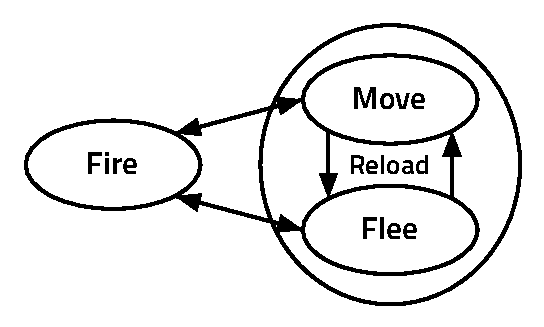
\includegraphics[width=5.5cm]{images/simple_unit_fight_FSM.pdf}
\end{center}
\caption{Fight FSM of a simple unit model: Heuristic Only AI (HOAI), which will serve as a baseline for benchmarks.}
\label{fig:fight_FSM}
\end{figure}


\subsection{Units Group}

\label{section:unitsgroup}
The units group (\texttt{UnitsGroup}, see Fig.~\ref{fig:conceptMICRO}) makes the shared \textit{future damage} data structure available to all units taking part in a fight. Units control is not limited to fight. As it is adversarial, it is perhaps the hardest task, but units control problems comprehends efficient team manoeuvering and other behaviors such as scouting of staying in position (formation). The units group structure helps for all that: it decides of the modes in which the unit has to be. We implemented 4 modes in our Bayesian unit (see Fig.~\ref{fig:unit_HFSM}): \textit{fight, move, scout, inposition}. When given a task, also named goal, by the tactician model (see Fig.~\ref{conceptMICRO}), the units group has to transform the task objective into sensory inputs for the units. 
\begin{itemize}
    \item In \textit{scout} and \textit{move} modes, the objective is extracted for the pathfinder output: it consists in key waypoints near the units. 
    \item In the \textit{inposition} mode, the objective is the final unit formation position. 
    \item In \textit{fight} mode, the objective depends of the confidence of the units group in the outcome of the battle. 
\begin{itemize}
    \item If the units group is outnumbered (in adjusted strength) and the task is not a suicidal one, the units group will ``fall back'' and give objectives towards retreat. 
    \item If the fight is even or manageable, the units group will not give any objective to units, which will set their own objectives either to their priority targets in \textit{fightMove()} or towards fleeing damages (towards highest potential damages gradient) in \textit{flee()}.
    \item If the units group is very confident in winning the fight, the objectives sensory inputs of the units will be set at the task objectives waypoints (from the pathfinder).
\end{itemize}
\end{itemize} 

\section{A Bayesian Model for Units Control}

\subsection{Bayesian Unit}

We use Bayesian programming as an alternative to logic, transforming incompleteness of knowledge about the world into uncertainty. In the case of units management, we have mainly \textit{intensional} uncertainty. Instead of asking questions like: where are other units going to be 10 frames later? Our model is based on rough estimations that are not taken as ground facts. Knowing the answer to these questions would require for our own (allied) units to communicate a lot and to stick to their plan (which does not allow for quick reaction nor adaptation). 

We propose to model units as sensory-motor robots described within the Bayesian robot programming framework \citep{Lebeltel04}. A Bayesian model uses and reasons on distributions instead of predicates, which deals directly with uncertainty. %Basically, a Bayesian unit will be attracted or repulsed by its sensory inputs. 
Our Bayesian units are simple hierarchical finite states machines (states can be seen as modes) that can scout, fight and move (see Figure~\ref{fig:unit_HFSM}). Each unit type has a reload rate and attack duration, so their fight mode will be as depicted in Figure~\ref{fig:fight_FSM} and Algorithm~\ref{alg:fight_FSM}. The difference between our simple HOAI presented above and Bayesian units are in \textit{flee()} and \textit{fightMove()} functions.
\begin{figure}[h]
\begin{center}
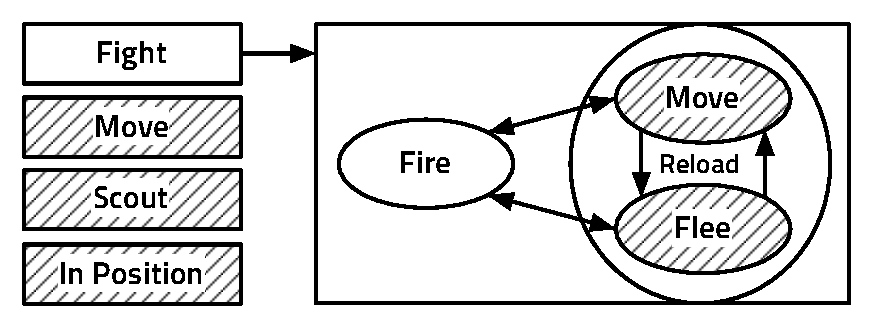
\includegraphics[width=7cm]{images/unit_HFSM2.pdf}
\end{center}
\caption{Bayesian unit modal FSM, detail on the fight mode. Stripped modes are Bayesian.}
\label{fig:unit_HFSM}
\end{figure}

The unit needs to determine where to go when fleeing and moving during a fight, with regard to its target and the attacking enemies, while avoiding collisions (which results in blocked units and time lost) as much as possible. \textbf{We now present the Bayesian program used for \textit{flee()} and \textit{fightMove()}}, which differ only by what is inputed as objective:
\subsubsection{Variables}
\begin{itemize}
\item $Dir_{i \in \llbracket 0 \dots n\rrbracket } \in \{True, False\}$: at least one variable for each atomic direction the unit can go to. $\PP(Dir_i = True) = 1$ means that the unit will certainly go in direction $i$ ($\Leftrightarrow \vec{d_i}$). For example, in StarCraft we use the 24 atomic directions (48 for the smallest and fast units as we use a proportional scale) plus the current unit position (stay where it is) as shown in Figure~\ref{fig:sc_fight}. %We could use one variable with 24 directions, the approach would be the same. %%% Note that $i \in \llbracket 0 \dots n\rrbracket \Leftrightarrow \mathbf{D}[i] \in \mathbf{D}$.

\item $Obj_{i \in \llbracket 0 \dots n\rrbracket } \in \{True, False\}$: adequacy of direction $i$ with the objective (given by a higher rank model). In our StarCraft AI, we use the scalar product between the direction $i$ and the objective vector (output of the pathfinding) with a minimum value ($0.3$ in \textit{move} mode for instance) so that the probability to go in a given direction is proportional to its alignment with the objective.
\begin{itemize}
    \item For \textit{flee()}, the objective is set in the direction which flees the potential damage gradient (corresponding to the unit type: ground or air).
    \item For \textit{fightMove()}, the objective is set (by the units group) either to retreat, to fight freely or to march aggressively towards the goal (see \ref{section:unitsgroup}).
\end{itemize}

\item $Dmg_{i \in \llbracket 0 \dots n\rrbracket } \in \{no, low, medium, high\}$: potential damage value in direction $i$, relative to the unit base health points, in direction $i$. In our StarCraft AI, this is directly drawn from two constantly updated potential damage maps (air, ground). %For instance, it allows our scouting units to avoid potential attacks as much as possible.

\item $A_{i \in \llbracket 0 \dots n\rrbracket } \in \{free, small, big\}$: occupation of the direction $i$ by an allied unit. The model can effectively use many values (other than ``occupied/free'') because directions may be multi-scale (for instance we indexed the scale on the size of the unit) and, in the end, small and/or fast units have a much smaller footprint, collision wise, than big and/or slow. In our AI, instead of direct positions of allied units, we used their (linear) interpolation $\frac{\mathrm{dist}(unit, \vec{d_i})}{unit.speed}$ (time it takes the unit to go to $\vec{d_i}$) 
frames later (to avoid squeezing/expansion).

\item $E_{i \in \llbracket 0 \dots n\rrbracket } \in \{free, small, big\}$: occupation of the direction $i$ by an enemy unit. As above.

\item $Occ_{i \in \llbracket 0 \dots n\rrbracket } \in \{free, building, staticterrain\}$%(this could have been 2 variables or we could omit static terrain but we stay as general as possible): 
: Occupied, repulsive effect of buildings and terrain (cliffs, water, walls).
\end{itemize}

There is basically one set of (sensory) variables per perception in addition to the $Dir_i$ values. 

\subsubsection{Decomposition}

The joint distribution ($JD$) over these variables is a specific kind of fusion called inverse programming \citep{LeHy04}. The sensory variables are considered conditionally independent knowing the actions, contrary to standard naive Bayesian fusion, in which the sensory variables are considered independent knowing the phenomenon.
\begin{eqnarray}
&& \PP(Dir_{1:n}, Obj_{1:n}, Dmg_{1:n}, A_{1:n}, E_{1:n}, Occ_{1:n})\\
& = & JD = \prod_{i=1}^{n} \PP(Dir_i) \PP(Obj_i | Dir_i) \\
                    && \PP(Dmg_i | Dir_i) \PP(A_i | Dir_i) \\
                    && \PP(E_i | Dir_i) \PP(Occ_i | Dir_i)
\end{eqnarray}
We assume that the $i$ directions are independent depending on the action because dependency is already encoded in (all) sensory inputs. 

\subsubsection{Forms}

\begin{itemize}
\item $\PP(Dir_i)$ prior on directions, unknown, so unspecified/uniform over all $i$. $\PP(dir_i) = 0.5$.

\item $\PP(Obj_i | Dir_i)$ for instance, ``probability that this direction is the objective knowing that we go there'' $\PP(obj_i | dir_i) = threshold + (1.0-threshold)\times <\vec{o},\vec{d_i}>$. %$\PP(Obj_i = T | Dir_i = T)$ is very high (close to one) when rushing towards an objective, whereas it is far less important when fleeing. 
We could have different $thresholds$ depending on the mode, this was not the case in our hand-specified tables: $threshold = 0.3$. The right diagram on Figure~\ref{fig:BayesianUnit_perceptions} shows $\PP(Obj_i|Dir_i)$ for each for the possible directions (inside the thick big square boundaries of atomic directions) with red being higher probabilities.

\item $\PP(Dmg_i | Dir_i)$ probability of damages values in direction $i$ knowing this is the direction that we are headed to. $\PP(Dmg_i = high | Dir_i = T)$ has to be small in many cases for the unit to avoid going to positions it could be killed instantly. Probability table:\\
\begin{center}
\begin{tabular}{|l|c|c|}
\hline
$Dmg_i$ & $dir_i$ & $\bar{dir_i}$ \\
\hline
no & 0.9 & 0.25 \\
low & 0.06 & 0.25 \\
medium & 0.03 & 0.25 \\
high & 0.01 & 0.25 \\
\hline
\end{tabular}
\end{center}

\item $\PP(A_i | Dir_i)$ probability that there is an ally in direction $I$ knowing this is the unit direction. It is used to avoid collisions by not going where allied units could be in the near future. Probability table:\\
\begin{center}
\begin{tabular}{|l|c|c|}
\hline
$A_i$ & $dir_i$ & $\bar{dir_i}$ \\
\hline
free & 0.9 & 0.333 \\
small & 0.06 & 0.333 \\
big & 0.03 & 0.333 \\
\hline
\end{tabular}
\end{center}
 

\item $\PP(E_i | Dir_i)$ same explanation and use as above but with enemy units, it can have different parameters as we may want to be stucking enemy units, or avoid them (mostly depending on the unit type). In a repulsive setting (what we mostly want), the left diagram in Figure~\ref{fig:BayesianUnit_perceptions} can be seen as $\PP(A_i,E_i | \bar{Dir_i})$ if red corresponds to high probabilities ($\PP(A_i,E_i|Dir_i)$ if red corresponds to lower probabilities). In our hand-specified implementation, for \textit{flee()} and \textit{fightMove()}, this is the same probability table as above (for $\PP(A_i | Dir_i)$).

\item $\PP(Occ_i | Dir_i)$ probability table that there is a blocking building or terrain element is some direction, knowing this is the unit direction, $\PP(Occ_i = Static | Dir_i = T)$ will be very low, whereas $\PP(Occ_i = Building | Dir_i = T)$ will also be very low but triggers building attack (and destruction) when there are no other issues.
Probability table:\\
\begin{center}
\begin{tabular}{|l|c|c|}
\hline
$Occ_i$ & $dir_i$ & $\bar{dir_i}$ \\
\hline
free & 0.999899 & 0.333 \\
building & 0.001 & 0.333 \\
static & 0.000001 & 0.333 \\
\hline
\end{tabular}
\end{center}

\end{itemize}

%%% TODO height: 0.2, 0.3, 0.45, 0.05 for normal/high/very high/unknown P(H_i|Dir_i)

%%% TODO learn exponential P(Dmg_i | Dir_i)
%%% TODO flock = Beta(\alpha, \beta), \beta > \alpha > 1 


\subsubsection{Identification}

Parameters and probability tables can be learned through reinforcement learning \citep{Sutton,Asmuth09} by setting up different and pertinent scenarii and search for the set of parameters that maximizes a reward function (more about that in the discussion). In our current implementation, the parameters and probability table values are hand specified.

\subsubsection{Question}

When in $fightMove()$, the unit asks:
\begin{small}
$$\PP(Dir_{1:n} | Obj_{1:n}, Dmg_{1:n}, A_{1:n}, E_{1:n}, Occ_{1:n}, Prio_{1:n})$$
\end{small}
When in $flee()$ or while moving or scouting (different balance/parameters), the unit asks:
$$\PP(Dir_{1:n} | Obj_{1:n}, Dmg_{1:n}, A_{1:n}, E_{1:n}, Occ_{1:n})$$
When flocking, the unit asks:
\begin{small}
$$\PP(Dir_{1:n} | Obj_{1:n}, Dmg_{1:n}, A_{1:n}, E_{1:n}, Occ_{1:n}, Att_{1:n,1:m}) $$
\end{small}
From there, the unit can either go in the most probable $Dir_i$ or sample through them. We describe the effect of this choice in the next section (and in Fig.~\ref{fig:BayesianUnitChoice}). A simple Bayesian fusion from 3 sensory inputs is shown in Figure~\ref{fig:BayesianUnitExample}, in which the final distribution on $Dir$ peaks at places avoiding damages and collisions while being towards the goal. Here follows the full Bayesian program of the model (\ref{bp:BayesianUnit_move}):

\begin{figure}[h]
\begin{center}
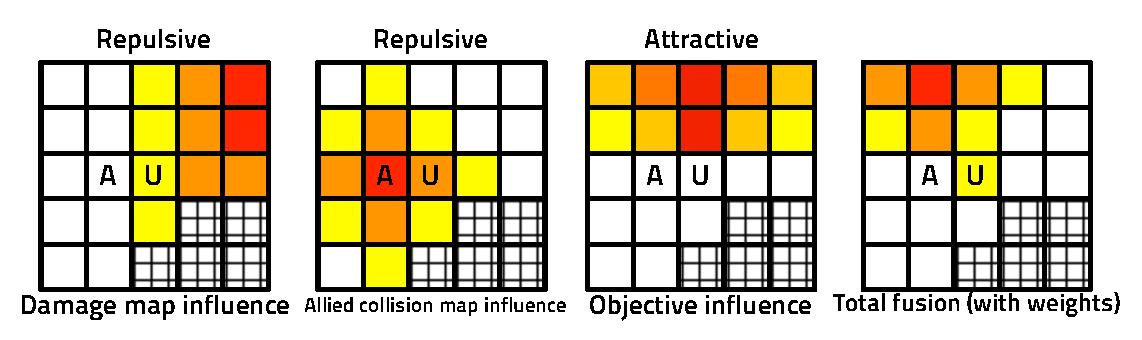
\includegraphics[width=13cm]{images/example_BayesianUnit.pdf}
\end{center}
\caption{Simple example of Bayesian fusion from 3 sensory inputs (damages and collisions avoidance, goal attraction). The grid pattern represents statically occupied terrain, the unit we control is in \texttt{U}, an allied unit is in \texttt{A}. The result is displayed on the rightmost image.}
\label{fig:BayesianUnitExample}
\end{figure}

\begin{figure}[!h]
\begin{eqnarray*}
\begin{sideways}\parbox{35mm}{\hspace{-1.3cm}Bayesian program}\end{sideways}
\begin{cases}
\begin{sideways}\parbox{15mm}{\hspace{-0.8cm}Description}\end{sideways}
    \begin{cases}
\begin{sideways}\parbox{18mm}{\hspace{-1.1cm}Specification ($\pi$)}\end{sideways}
        \begin{cases}
        Variables\\
Dir_{1:n}, Obj_{1:n}, Dmg_{1:n}, A_{1:n}, E_{1:n}, Occ_{1:n} \\
        Decomposition\\
 \PP(Dir_{1:n}, Obj_{1:n}, Dmg_{1:n}, A_{1:n}, E_{1:n}, Occ_{1:n}) =  \prod_{i=1}^{n} \big[ \PP(Dir_i) \\
 \PP(Obj_i | Dir_i) \PP(Dmg_i | Dir_i) \PP(A_i | Dir_i) \PP(E_i | Dir_i) \PP(Occ_i | Dir_i)\big]\\
        Forms\\
\PP(Dir_i): \mathrm{prior\ on\ directions\ (crossing\ policy)} \\
\PP(XYZ_i | Dir_i):\ \mathrm{probability\ tables}\\
        \end{cases}\\
    Identification\ (using\ \delta)\\
\mathrm{reinforcement\ learning\ or\ hand\ specified\ (or\ distribs.\ parameters\ optimization)}
    \end{cases}\\
Question\\
 \mathrm{fight moving:}\ \ \PP(Dir_{1:n} | Obj_{1:n}, Dmg_{1:n}, A_{1:n}, E_{1:n}, Occ_{1:n}, Prio_{1:n})\\
 \mathrm{fleeing:}\ \  \PP(Dir_{1:n} | Obj_{1:n}, Dmg_{1:n}, A_{1:n}, E_{1:n}, Occ_{1:n})\\
 \mathrm{flocking:}\ \  \PP(Dir_{1:n} | Obj_{1:n}, Dmg_{1:n}, A_{1:n}, E_{1:n}, Occ_{1:n}, Att_{1:n,1:m})\\
\end{cases}
\end{eqnarray*}
\label{bp:BayesianUnit_move}
\end{figure}

\subsubsection{Move}
\textbf{Without flocking}\\
\textbf{With flocking}\\
\subsubsection{Scout}
\subsubsection{In position}

There are additional variables for specific modes/behaviors:
\begin{itemize}
\item $Prio_{i \in \llbracket 0 \dots n\rrbracket } \in \{True, False\}$: combined effect of the priority targets that attract the unit while in fight ($fightMove()$). The $JD$ is modified as $JD \times \Pi_{i=1}^{n} \PP(Prio_i | Dir_i)$, where $\PP(Prio_i | Dir_i)$ is a probability table, that corresponds to the attraction of a priority (maybe out of range) target in this direction. This is efficient to be able to target casters or long range units for instance.

\item $Att_{i \in \llbracket 0 \dots n\rrbracket, j \in \llbracket 0 \dots m \rrbracket}$: allied units attractions and repulsions to produce a \textit{flocking} behavior while moving. Different than $A_i$, the $JD$ would become $JD \times \Pi_{i=1}^{n} \Pi_{j=1}^{m} \PP(Att_{i,j} | Dir_i)$, where $\PP(Att_{i,j} | Dir_i)$ is a probability table for flocking: a too close unit $j$ will repel the Bayesian unit ($\PP(Att_{i,j} | Dir_i) < mean$) whereas another unit $j$ will attract depending on its distance (and possibly, leadership).

\item $Dir_{i \in \llbracket 0 \dots n\rrbracket }^{t-1} \in \{True, False\}$: the previous selected direction, $Dir_i^{t-1} = T$ iff the unit went to the direction $i$, else $False$ for a steering (smooth) behavior. The $JD$ would then be $JD \times \Pi_{i=1}^{n} \PP(Dir_i^{t-1} | Dir_i)$, with $\PP(Dir_i^{t-1} | Dir_i)$ the influence of the last direction, either a table or a parametrized Bell shape over all the $i$.

\item One can have a distribution over a $n$ valued variable $Dir \in \{D\}$. (Each set of boolean random variable can be seen as a $|D|$ valued variable.) The $JD$ would then be $JD \times \PP(Dir).\Pi_{i=1}^{n} \PP(Dir_i | Dir)$.
\end{itemize}



\section{Results on StarCraft}
StarCraft micro-management involves ground, flying, ranged, contact, static, moving (at different speeds), small and big units (see Figure~\ref{fig:sc_fight}). Units may also have splash damage, spells, and different types of damages whose amount will depend on the target size. It yields a rich states space and needs control to be very fast: human progamers can perform up to 400 ``actions per minute'' in intense fights. The problem for them is to know which actions are effective and the most rewarding to spend their actions efficiently. A robot does not have such physical limitations, but yet, badly chosen actions have negative influence on the issue of fights. %The problem is to identify what has to be done and what can be done, in real-time.

\subsection{Our Robot Architecture}

Our full robot has separate agents types for separate tasks (strategy, tactics, economy, army, as well as enemy estimations and predictions): the part that interests us here, the unit control, is managed by Bayesian units directly. Their objectives are set by military goal-wise atomic units group, themselves spawned to achieve tactical goals (see Fig.~\ref{fig:conceptMICRO}). Units groups tune their Bayesian units modes (scout, fight, move) and give them $Obj_i$ as sensory inputs. The Bayesian unit is the smallest entity and controls individual units as sensory-motor robots according to the model described above. The only inter Bayesian units communication about attack targets is handled by a structure shared at the units group level.

\subsection{Experiments}

Our implementation\footnote{\textsc{BroodwarBotQ}, code and releases: \url{http://github.com/SnippyHolloW/BroodwarBotQ}} (BSD licensed) uses BWAPI\footnote{BWAPI: \url{http://code.google.com/p/bwapi/}} to get information from and to control StarCraft. 
We produced three different AI to run experiments with, along with the original AI (OAI) from StarCraft:
\begin{itemize}
\item Heuristic only AI (HOAI), section~4.1: this AI shares the target selection heuristic with our other AI and will be used as a dummy reference (in addition to StarCraft original AI) to avoid bias due to the target selection heuristic.
\item Bayesian AI picking best (BAIPB): this AI follows the model of section~4.2 and selects the most probable $Dir_i$ as movement. 
\item Bayesian AI sampling (BAIS): this AI follows the model of section~4.2 and samples through $Dir_i$ according to their probability ($\Leftrightarrow$ according to $Dir$ distribution).
\end{itemize}

The experiments consisted in having the AIs fight against each others on a micro-management scenario with mirror matches of 12 and 36 ranged ground units (Dragoons). In the 12 units setup, the unit movements during the battle is easier (less collision probability) than in the 36 units setup. We instantiate only the army manager (no economy in this special maps), one units group manager and as many Bayesian units as there are units provided to us in the scenario. The results are presented in Table~\ref{tab:win_ratios}.

\definecolor{grey}{rgb}{0.7,0.7,0.7}
\begin{table}[h]
\begin{center}
\begin{tabular}{l|c|c|c|c}
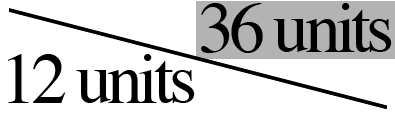
\includegraphics[width=1.5cm]{images/array_top2.png} & OAI & HOAI & BAIPB & BAIS \\
\hline
OAI & (50\%) & \colorbox{grey}{64\%} & \colorbox{grey}{9\%} & \colorbox{grey}{3\%} \\
HOAI & 59\% & (50\%) & \colorbox{grey}{11\%} & \colorbox{grey}{6\%} \\
BAIPB & 93\% & 97\% & (50\%) & \colorbox{grey}{3\%} \\
BAIS & 93\% & 95\% & 76\% & (50\%)
\end{tabular}
\end{center}
% BAIPB+Heuristics flee/fightmove 12 goons vs OAI 94/100
% BAIPB+Heuristics flee/fightmove 36 goons vs OAI 95/100
% pure BAIPB (fightMove only on ``potential fields'') 12 goons vs OAI 51/33
% pure BAIPB (fightMove only on ``potential fields'') 36 goons vs OAI 10/16
%%%\caption{Win ratios over at least 200 battles of the Original AI (OAI), Heuristic Only AI (HOAI), Bayesian AI Pick Best (BAIPB) and Bayesian AI Sample (BAIS) in two mirror setups: 12 and 36 ranged units. Read line vs column: for instance HOAI won 59\% of its matches against OAI in the 12 units setup. Note: The average amount of units left at the end of battles is proportional to the percentage of wins.}
\caption{Win ratios over at least 200 battles of OAI, HOAI, BAIPB and BAIS in two mirror setups: 12 and 36 ranged units. Read line vs column: for instance HOAI won 59\% of its matches against OAI in the 12 units setup. Note: The average amount of units left at the end of battles is grossly proportional to the percentage of wins.}
\label{tab:win_ratios}
\end{table}

These results show that our heuristic (HAOI) is comparable to the original AI (OAI), perhaps a little better, but induces more collisions. For Bayesian units however, the ``pick best'' (BAIPB) direction policy is very effective when battling with few units (and few movements because of static enemy units) as proved against OAI and HOAI, but its effectiveness decreases when the number of units increases: all units are competing for the best directions (to $flee()$ or $fightMove()$ in) and they collide. The sampling policy (BAIS) has way better results in large armies, and significantly better results in the 12 units vs BAIPB, supposedly because BAIPB moves a lot (to chase wounded units) and collide with BAIS units. Sampling entails that the competition for the best directions is distributed among all the ``bests to good'' wells of well-being, from the units point of view. We also ran tests in setups with flying units in which BAIPB fared as good as BAIS (no collision for flying units) and way better than OAI.

We had a tie with the winner of AIIDE 2010 StarCraft micro-management competition, winning with ranged units and losing with contact units. %%% TODO

\subsection{Uses and extensions}
This model is currently at the core of the micro-management of our StarCraft bot. We use it mainly with four modes corresponding to four behaviors (four sets of parameters):
\begin{itemize}
\item Scout: in this mode, the (often quick and low hit points) unit avoids danger by modifying locally its pathfinding-based, objectives oriented route to avoid damages according to $\PP(Dmg_i|Dir_i)$.
\item In position: in this mode, the unit try to keep its ground but can be ``pushed'' by other units wanting to pass through with $\PP(A_i | Dir_i)$. This is useful at a tactical level to do a wall of units that our units can traverse but the opponent's cannot. Basically, there is an attraction to the position of the unit and a stronger repulsion of the interpolation of movements of allied units.
\item Flock: in this mode, our unit moves influenced by other allied units through $\PP(Att_{i \in \llbracket 0 \dots n\rrbracket, j \in \llbracket 0 \dots m \rrbracket})$ that repulse or attract it depending on its distance to the interpolation of the allied unit $j$. It allows our units to move more efficiently by not splitting around obstacles and colliding less.
\item Fight: in this mode, our unit will follow the damages gradient to smart positions, for instance close to tanks (they cannot fire too close to their position) or far from too much contact units if our unit can attack with range. Our unit moves are also influenced by its priority targets, its goal (go through a choke, flee, etc.) and other units.
\end{itemize}

This model can be used to specify the behavior of units in RTS games. Instead of relying on a ``units push each other'' physics model for handling dynamic collision of units, this model makes the units react themselves to collision in a more realistic fashion (a marine cannot push a tank, the tank will move). The realism of units movements can also be augmented with a simple-to-set $\PP(Dir^{t-1}|Dir^t)$ steering parameter, although we do not use it in the competitive setup.



\section{Discussion}

\subsection{Perspectives}
%%% Conclusion and perspectives: opens the game to parameters learning, RL and/or EA (Bayesian fusion FTW!)
If we learn the parameters of such a model to mimic existing data (data mining) or to maximize a reward function (reinforcement learning), we can interpret the parameters that will be obtained more easily than parameters of an artificial neural network for instance. Parameters learned in one setup can be reused in another if they are understood. We claim that specifying or changing the behavior of this model is much easier than changing the behavior generated by a FSM, and game developers can have a fine control over it. Dynamic switches of behavior (as we do between the scout/flock/inposition/fight modes) are just one probability tables switch away. In fact, probability tables for each sensory input (or group of sensory inputs) can be linked to sliders in a ``behavior editor'' and game makers can specify the behavior of their units by specifying the degree of effect of each perception (sensory input) on the behavior of the unit and see the effect in real time. This is not restricted to RTS and could be applied to \glos{RPG} and even \glos{FPS} \gloss{gameplay}.


Future work could consist in using reinforcement learning \citep{Sutton} or evolutionary algorithms \citep{SmithCIG10} to learn the probability tables. It should enhance the performance of our Bayesian units in specific setups. It implies making up challenging scenarii and dealing with huge sampling spaces \citep{Asmuth09}. Also, we could use multi-modality \citep{Colas10} and inverse programming \citep{LeHy04} to get rid of the remaining (small: fire-retreat-move) FSM. Also, there are yet many collision cases that remain unsolved (particularly visible with contact units like Zealots and Zerglings), so we could also try: 
\begin{itemize}
\item adding local priority rules to solve collisions (for instance through an asymmetrical $\PP(Dir_i^{t-1}|Dir_i)$) that would entails units crossing lines with a preferred side (some kind of ``social rule''),
\item use a units group level supervision using Bayesian units' distributions over $Dir$ as preferences or constraints (for a solver),
\item use $\PP(Dir)$ as an input to another Bayesian model at the units group level of reasoning.
\end{itemize}

\begin{figure}[h]
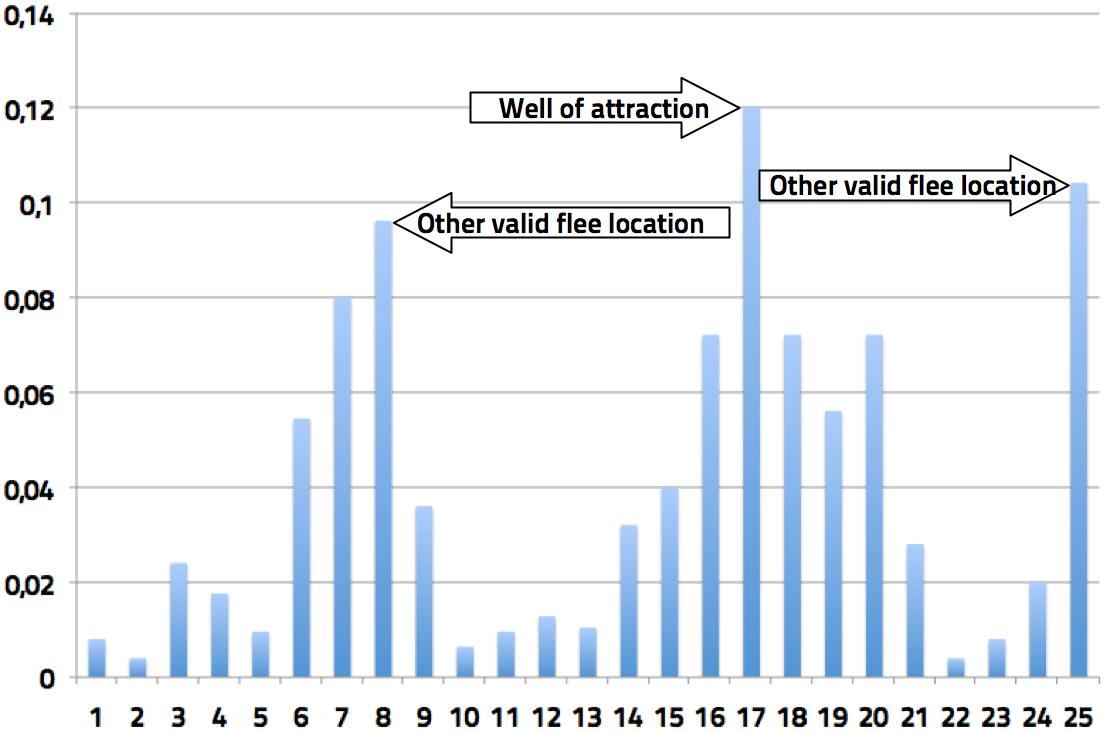
\includegraphics[width=12cm]{images/distDir.png}
\hspace{0.8cm}
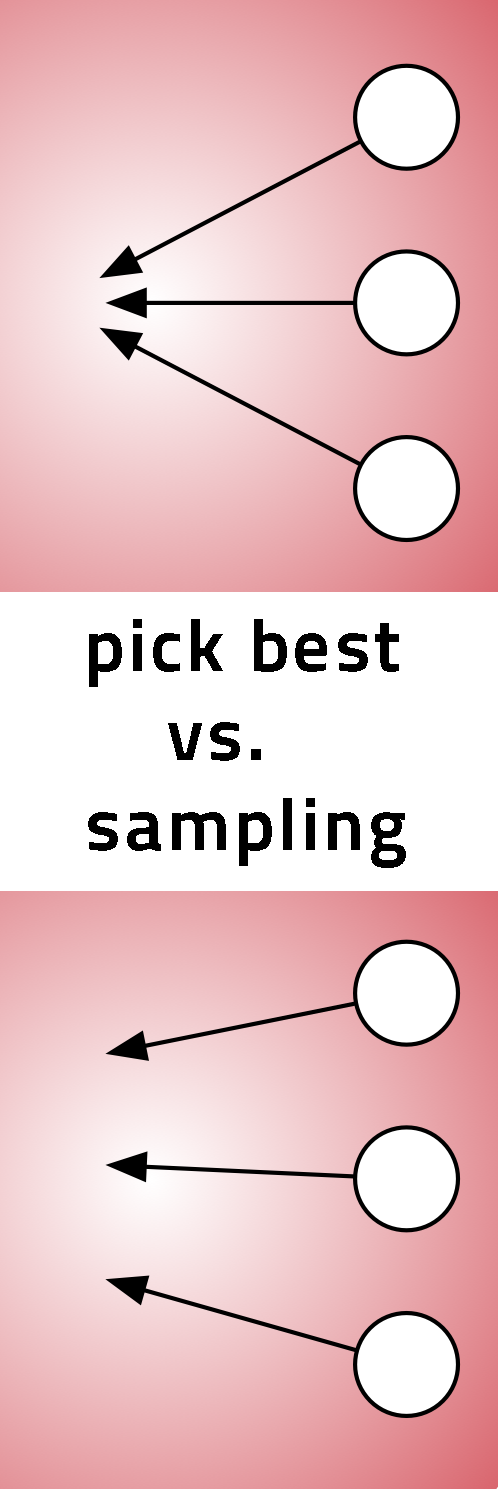
\includegraphics[width=2.6cm]{images/flee_sample.png}
\caption{Example of $\PP(Dir)$ when fleeing, showing why sampling (BAIS, bottom graphic on the right) may be a better instead of picking the most best direction (BAIPB, here $Dir=17$ in the plot, top graphic on the right) and triggering units collisions.}
\label{fig:BayesianUnitChoice}
\end{figure}
\label{BayesianUnitCCL}
Finally, there are still two points on which our reactive \textit{decentralized} model can be challenged with ``optimality'':
\begin{itemize}
    \item local optimum which could stuck units: concave (strong) repulsors (static terrain, very high damage field) could trap our reactive, small look-ahead unit. A pragmatic solution to that is to remember that the $Obj$ sensory inputs come from the pathfinder and have its influence to grow when in difficult situations (not moved for a long time, concave shape detected...). Another solution is inspired by ants: simply release a repulsive field (a repulsive ``pheromone'') behind the unit and it will be repulsed by places it already visited instead of oscillating around the local optima (see Fig.~\ref{fig:BayesianTrailingPheromone}).
    \item collision due to concurrency for ``best'' positions: as seen in Figure.~\ref{fig:BayesianUnitChoice}, units may compete for a well of potential. The solution that we use is to sample in the $Dir$ distribution, which gives better results than picking the most probable direction as soon as there are many units. Another solution, inspired by \citep{Marthi05concurrenthierarchical}, would be for the Bayesian units to communicate their $Dir$ distribution to the units group which would give orders that optimize either the sum of probabilities, or the minimal discrepancy in dissatisfaction, or the survival of costly units (as shown in Fig.~\ref{fig:BayesianUnitsGroup})...
\end{itemize}



The sensory inputs given to a ``Bayesian unit'' controls its objective(s) or goal(s) and the parametrization of his probabilistic model controls its behavior and degree of freedom. As an illustration (only), two of the extreme cases are $\PP(Direction=x|Objective=x)=1$: no freedom, $\PP(Direction=x|Objective=y)=\PP(Direction=x)$: no influence of the objective. %%% TODO

In general, if one decides to cover a lot of space with directions (\textit{i.e.} have more than just atomic directions, \textit{i.e.} use this model for planning), one needs to consider directions whose paths collide with each others. For instance, a $\vec{d_i}$ far from the unit can force the unit to go through a wall of allied units ($A_j = Big$) or potential damages. %%% TODO

\subsection{Conclusion}
We have implemented this model in StarCraft, and it outperforms the original AI as well as other bots. Our approach does not require vertical integration of higher level goals, as opposed to CBR and reactive planning \citep{Ontanon2007,WeberCIG10}, it can have a completely different model above feeding sensory inputs like $Obj_i$. It scales well with the number of units to control thanks to the absence of communication at the unit level, and is more robust and maintainable than a FSM.
